\documentclass[10pt]{article}
\usepackage{verbatim, amsmath,amssymb,amsthm}
\usepackage[margin=.5in,nohead,nofoot]{geometry}
\usepackage{sectsty}
\usepackage{float,graphicx}
\sectionfont{\normalsize}
\subsectionfont{\small}
\subsubsectionfont{\footnotesize}


\title{GRB Classification - June 6, 2010}
\date{}
\author{James Long}
\newtheorem{theorem}{Theorem}[section]
\newtheorem{definition}{Definition}[section]
\newtheorem{example}{Example}[section]

\newcommand{\argmin}[1]{\underset{#1}{\operatorname{argmin}}\text{ }}
\newcommand{\argmax}[1]{\underset{#1}{\operatorname{argmax}}}
\newcommand{\minimax}[2]{\argmin{#1}\underset{#2}{\operatorname{max}}}
\newcommand{\bb}{\textbf{b}}

\newcommand{\Var}{\text{Var }}
\newcommand{\Cov}{\text{Cov }}


\newenvironment{my_enumerate}{
\begin{enumerate}
  \setlength{\itemsep}{1pt}
  \setlength{\parskip}{0pt}
  \setlength{\parsep}{0pt}}{\end{enumerate}
}



% Alter some LaTeX defaults for better treatment of figures:
    % See p.105 of ``TeX Unbound'' for suggested values.
    % See pp. 199-200 of Lamport's ``LaTeX'' book for details.
    %   General parameters, for ALL pages:
\renewcommand{\topfraction}{0.9}% max fraction of floats at top
\renewcommand{\bottomfraction}{0.8}% max fraction of floats at bottom
    %   Parameters for TEXT pages (not float pages):
    \setcounter{topnumber}{2}
    \setcounter{bottomnumber}{2}
    \setcounter{totalnumber}{4}     % 2 may work better
    \setcounter{dbltopnumber}{2}    % for 2-column pages
    \renewcommand{\dbltopfraction}{0.9}% fit big float above 2-col. text
    \renewcommand{\textfraction}{0.07}% allow minimal text w. figs
    %   Parameters for FLOAT pages (not text pages):
    \renewcommand{\floatpagefraction}{0.7}% require fuller float pages
    % N.B.: floatpagefraction MUST be less than topfraction !!
    \renewcommand{\dblfloatpagefraction}{0.7}% require fuller float pages

    % remember to use [htp] or [htpb] for placement





\begin{document}
\maketitle
\section{Introduction}

High redshift events are defined as redshifts greater than 4. There are 14 high redshift events and 118 low redshift events. There are a total of 76 features. There are 40 non error features and 36 error features. Many (all?) of the error features come in pairs. For example there is a feature A and then two associated error features A\_negerr and A\_poserr. Three features (bat\_is\_rate\_trigger, v\_mag\_isupper, and wh\_mag\_isupper) take the values yes / no. All other features are continuous.

We fit 6 CART classifiers to the data. There are three costs for misclassifying a high redshift event as a low redshift event: 3, 5, and 7. We apply these three costs to two feature sets: non-error features (40 in total) and all features (76 in total). In section \ref{sec:results} results are discussed. In \ref{sec:trees} trees are discussed and displayed.

\section{Results}
\label{sec:results}

Table \ref{tab:errors} displays cross validation error and the redshift value of misclassified high redshifts for each of the six classifiers. The cross validation errors are a bit opaque. With cross validation (specifically 10 fold cross validation), the observations are divided into 10 parts of roughly equal size. One part of the data is ``held out'' and the model is fit to the other 9 parts. Then the held out part is classified using this model. The error for this held out section is computed. This is repeated for each of the ten sections of the data. ``Error'' in this case in defined as:
\begin{equation}
\frac{\text{COST * (\# high as low)} + \text{1 * (\# low as high)}}{(\text{COST*\# high}) + (\text{\# low})} 
\end{equation}
I am not sure that this measurement of error is the best way to evaluate performance. Perhaps Tamara has suggestions on something better. Also, I ran the code several times and I am a bit worried about the variability of the cross validation estimate of error. I will try to get error bars on these so the numbers have more meaning.

For each of the 6 classifications, I included the redshift values of the high redshift events that were classified as low redshift under the notion that if most of the error of HIGH as LOW were of events in the 4 - 4.5 range this would be less bad than misclassifications in the redshift ranges of 5 and up. Also seeing which redshift were misclassified gives an idea of whether there is any sort of continuity in the feature space in the sense that one might expect high redshift events just over 4 to be difficult to classify because they are so close to the low redshift events and that as a result most of the misclassifications of high redshift events would occur in the 4-4.5 range. On repeated runs of the code there was a lot of variability in which high redshift were misclassified so do not treat these numbers as revealing any fundamental truths about GRBs.

% latex table generated in R 2.11.1 by xtable 1.5-6 package
% Sun Jun  6 15:17:20 2010
\begin{table}[H]
\begin{center}
\begin{tabular}{ccc}
  & Without Error Features & With Error Features \\ 
  \hline
Cost 3 & 0.731 & 0.694 \\ 
   & (6.6, 4, 4.3, 4.1, 4.4, 5.1, 8.1) & (6.6, 6.3, 5.3, 4, 4.9, 5.6, 4.3, 4.1, 6.7, 4.4, 8.1, 4.3) \\ 
   \hline
Cost 5 & 0.665 & 0.665 \\ 
   & (4, 4.9, 4.3, 4.1, 4.6, 4.4, 8.1) & (6.6, 6.3, 4, 4.9, 5.6, 4.3, 4.1, 4.6, 4.4) \\ 
   \hline
Cost 7 & 0.681 & 0.69 \\ 
   & (6.6, 6.3, 4, 4.3, 4.1, 4.4) & (6.6, 5.3, 4, 4.1, 4.6, 4.4) \\ 
   \hline
\end{tabular}
\caption{Performance of CART for Two Sets of Features and 3 Loss Functions}
\label{tab:errors}
\end{center}
\end{table}


\section{Trees}
\label{sec:trees}
Figures \ref{fig:noErrorCost3},  \ref{fig:noErrorCost5},  \ref{fig:noErrorCost7}, \ref{fig:ErrorCost3},  \ref{fig:ErrorCost5}, and \ref{fig:ErrorCost7} are the trees generated from the data with the three costs and two sets of features used in table \ref{tab:errors}. These are the trees fit on all the data, not on a cross validated portion of the data. However cross validation is built into the tree growing procedure so in most cases trees do not overfit the data. A new observation dropped into the tree will travel left at a node if the node expression is true, and right if the node expression is false. For example, all trees start with ``v\_mag\_isupper = yes'', so if a new observation has yes for ``v\_mag\_isupper'' then it will go to the left. The terminal nodes have an ``H'' if an observation landing in that node is classified as ``high'' and 'L' if it is classified as low. The two numbers separated by a forward slash at each terminal node are a bit confusing. The left number is the number of high GRB obserbations in that node \textit{times} the cost of misclassifying a high GRB as a low GRB. So in figure \ref{fig:noErrorCost3} the left most terminal node has an 'H' and ''33/10''. An observation falling into this node will be classified as high. 11 observations from the data in this node where high GRB events, and 10 were low GRB events. In general, if the number on the left of the forward slash is larger than the number on the right, the node will classify as ''H'', otherwise as ''L.'' 

Here are some observations on the trees. v\_mag\_isupper, A, and flx\_pc\_late are three important features. Most high gamma ray bursts have `yes' for v\_mag\_isupper. The two high redshift gamma ray bursts with no for v\_mag\_isupper have low FLX\_PC\_LATE. When v\_mag\_isupper is yes but A is high (greater than around -1.56) the event tends to be a low redshift GRB. Do these observations from the trees make scientific sense? We could definitely be picking up noise with some of these trees, especially nodes where there are 2 high redshift events. These trees are much more optimistic than the cross validation results in table \ref{tab:errors}. 

\subsection{No Error Features}

\begin{figure}[H]
\begin{center}

\includegraphics[height=5in,width=5in]{noErrorCost3.pdf}
\caption{Cost 3, no error features.\label{fig:noErrorCost3}}
\end{center}
\end{figure}


\begin{figure}[H]
\begin{center}
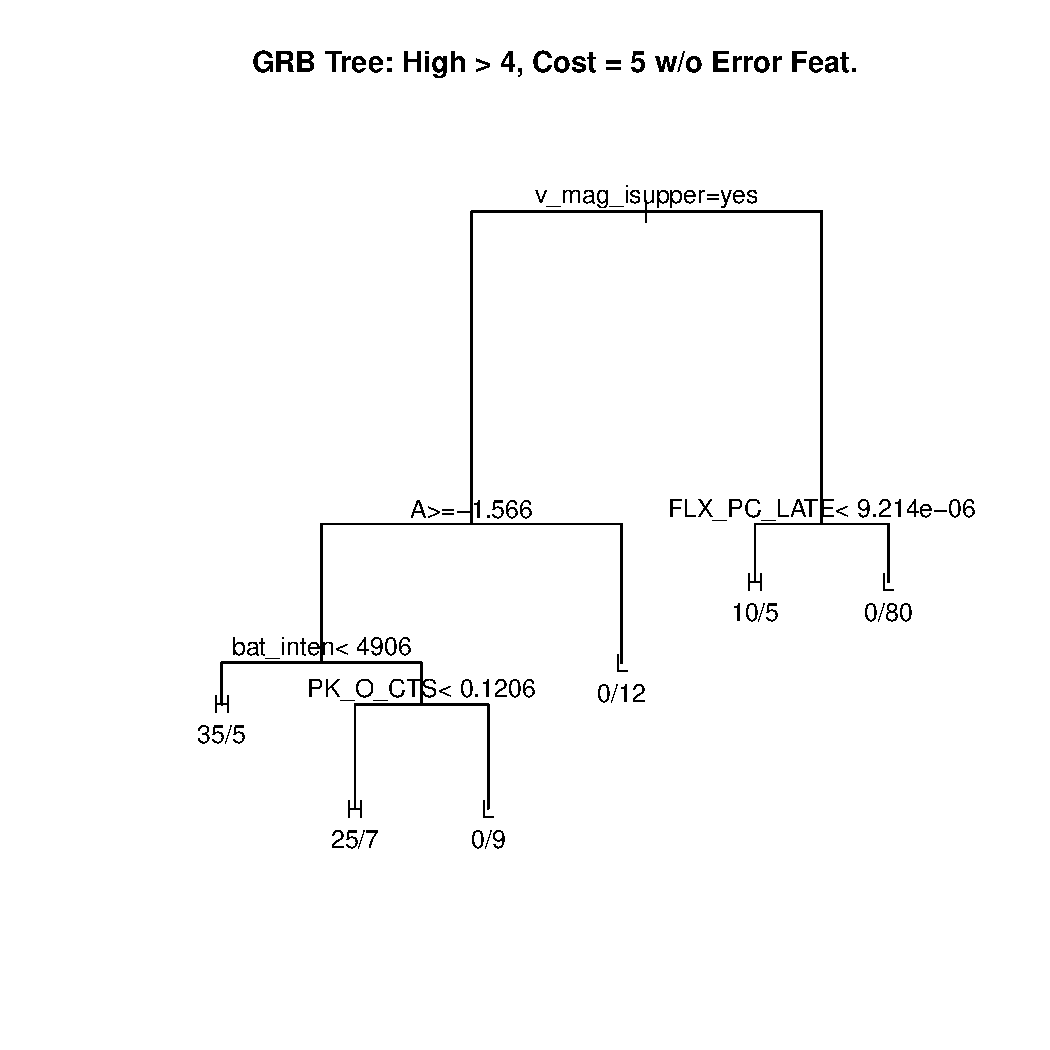
\includegraphics[height=5in,width=5in]{noErrorCost5.pdf}
\caption{Cost 5, no error features.\label{fig:noErrorCost5}}
\end{center}
\end{figure}



\begin{figure}[H]
\begin{center}
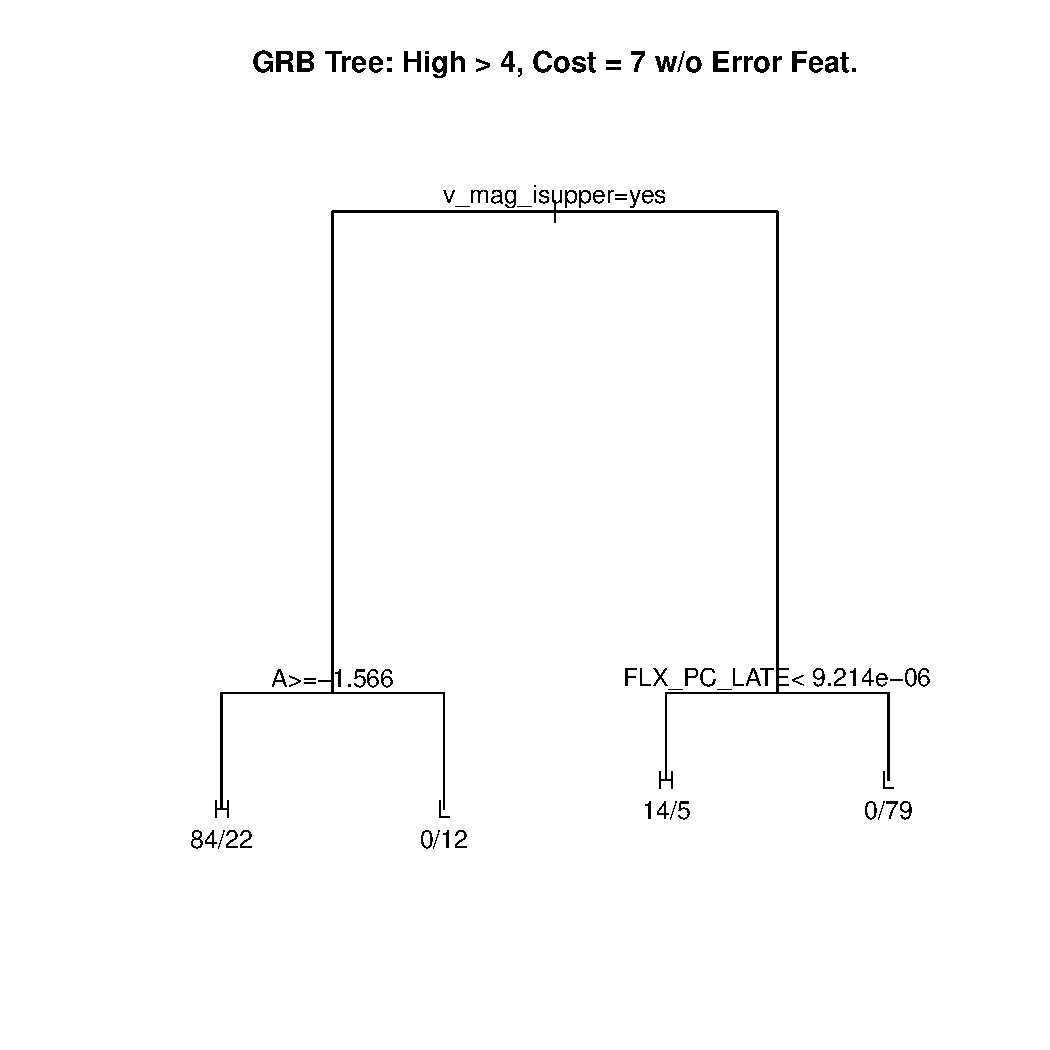
\includegraphics[height=5in,width=5in]{noErrorCost7.pdf}
\caption{Cost 7, no error features.\label{fig:noErrorCost7}}
\end{center}
\end{figure}





\subsection{With Error Features}

\begin{figure}[H]
\begin{center}
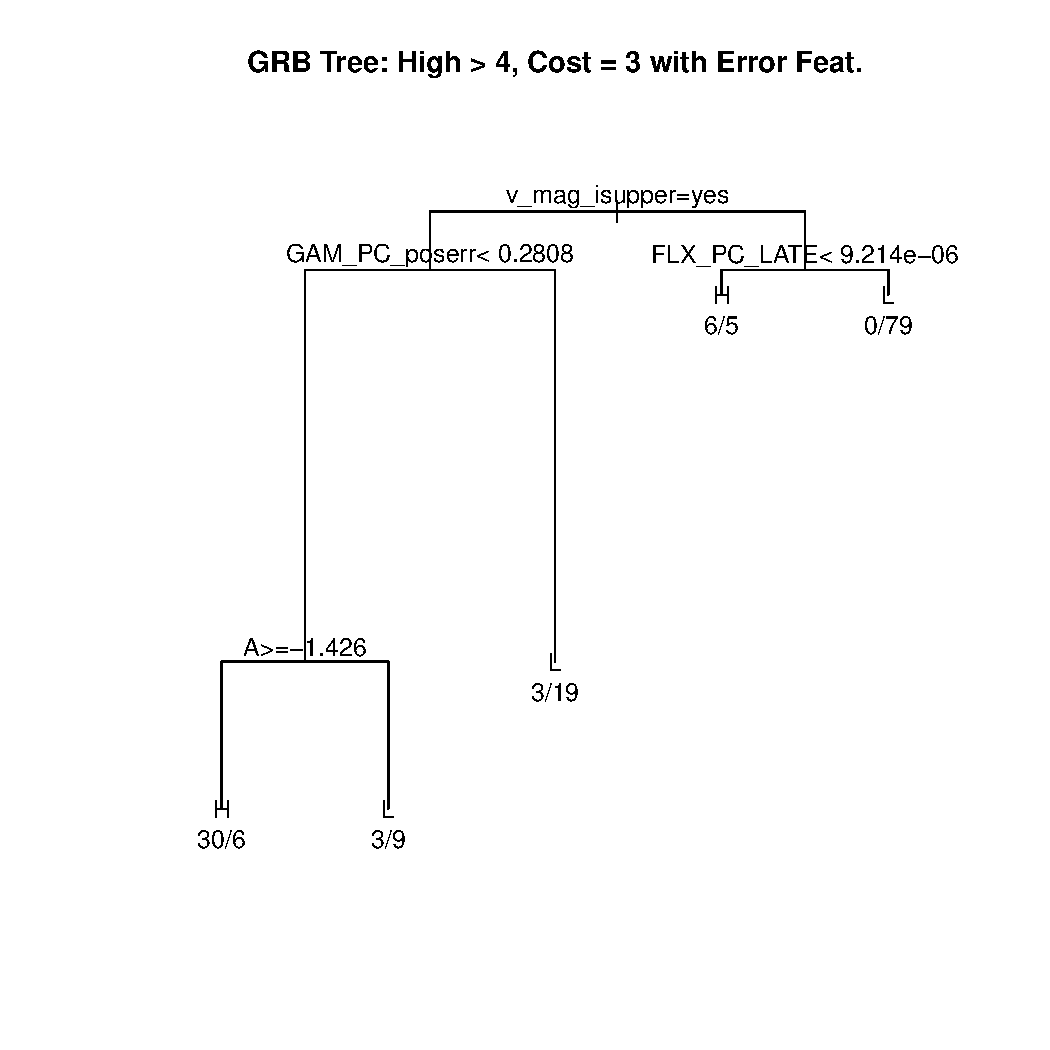
\includegraphics[height=5in,width=5in]{ErrorCost3.pdf}
\caption{Cost 3, with error features.\label{fig:ErrorCost3}}
\end{center}
\end{figure}


\begin{figure}[H]
\begin{center}
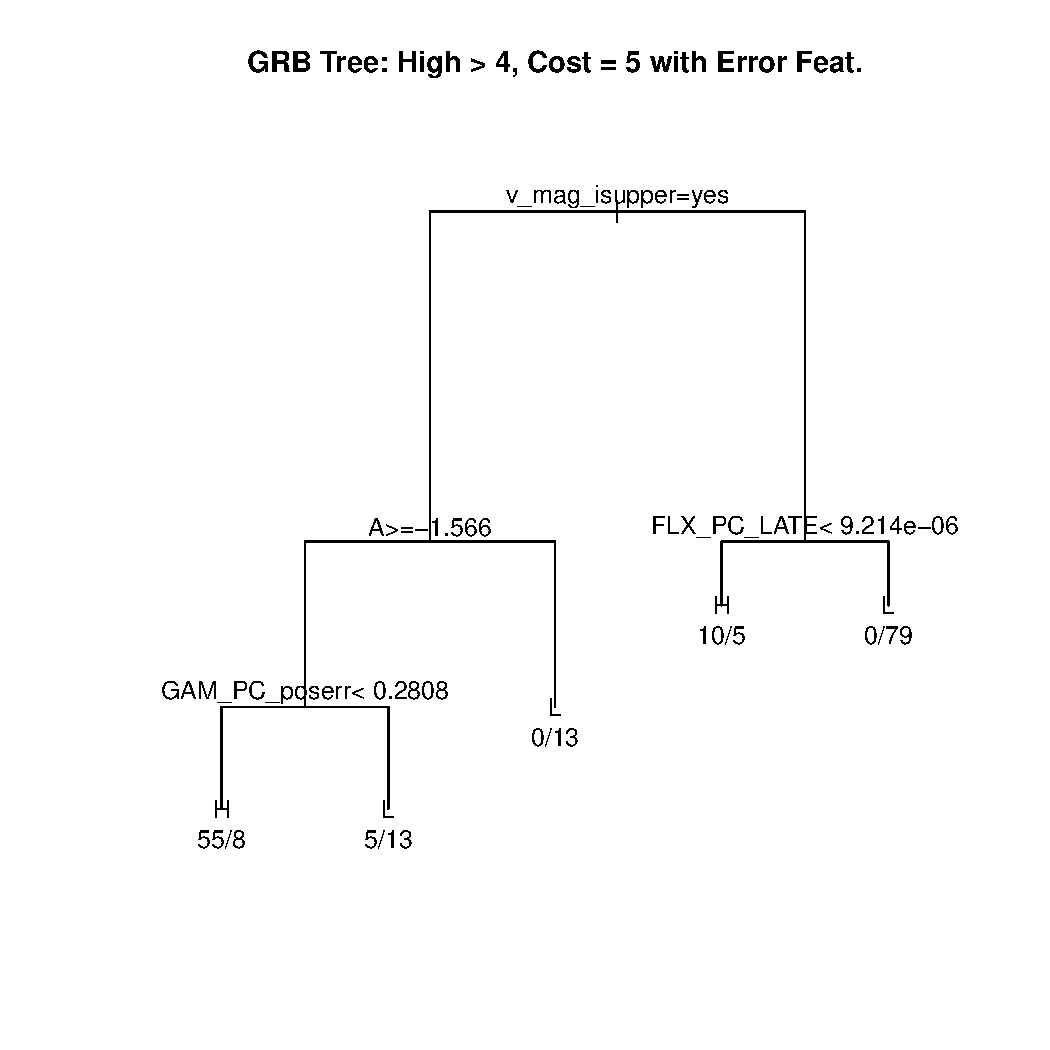
\includegraphics[height=5in,width=5in]{ErrorCost5.pdf}
\caption{Cost 5, with error features.\label{fig:ErrorCost5}}
\end{center}
\end{figure}



\begin{figure}[H]
\begin{center}
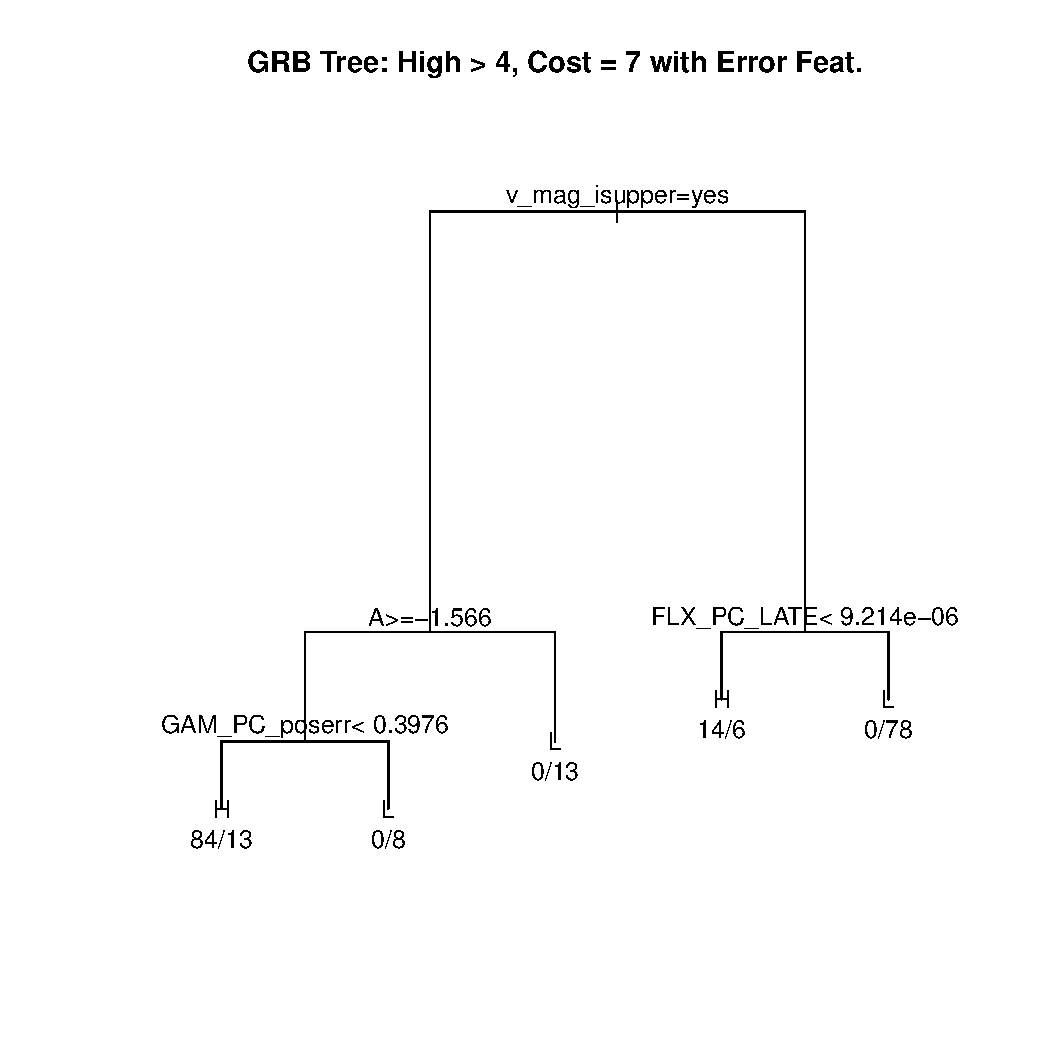
\includegraphics[height=5in,width=5in]{ErrorCost7.pdf}
\caption{Cost 7, with error features.\label{fig:ErrorCost7}}
\end{center}
\end{figure}


\section{Some Questions}
\begin{enumerate}
\item What is the difference between the t90 and T90 features?
\end{enumerate}

\end{document}
